\documentclass[12pt]{article}
\usepackage[utf8]{inputenc} % input encoding
\usepackage[T1]{fontenc} % Use an 8-bit font encoding, so that ã is a
                         % single glyph in the font. Yields better
                         % hyphenation and better cut-and-paste from pdf
\usepackage{times} % Comment this line you you want the default font, Computer Roman
% \usepackage[portuguese]{babel} % Uncomment this file you plan to write in Portuguese
\usepackage{hyperref}
\usepackage{listings}
\usepackage{graphicx}
\usepackage[section]{placeins}
\usepackage{multicol}
\usepackage{tabularx}
\usepackage{makecell}
\graphicspath{ {./images/} }
\sloppy

\lstset{frame=tb,
  aboveskip=3mm,
  belowskip=3mm,
  showstringspaces=false,
  columns=flexible,
  basicstyle={\small\ttfamily},
  numbers=none,
  breaklines=true,
  breakatwhitespace=true,
  tabsize=3
}

\title{TST JUnit Testing \\
  \Large Software Verification and Validation \\ 2019--2020
}
\author{
  João David\\49448
  \and
  Ye Yang\\49521
}
\date{09/05/2020}

\begin{document}
\maketitle

\section{Instruction Coverage}
\subsection{size()}
\begin{lstlisting}
    public int size() {
        return n; //I1
    }
\end{lstlisting}

\begin{table}[htb]
\centering
\begin{tabular}{| c | c | c | c |} 
 \hline
 Test Case & Values & Expected / Actual & IC\\ \hline
 sizeZeroTest & - & 0 & I1 \\ \hline

\end{tabular}
\end{table}

\subsection{contains(String key)}
\begin{lstlisting}
    public boolean contains(String key) {
        if (key == null)  //I1
            throw new IllegalArgumentException("argument to contains() is null"); //I2
        return get(key) != null; //I3
    }
\end{lstlisting}

\begin{table}[htb]
\centering
\begin{tabular}{| c | c | c | c |} 
 \hline
 Test Case & Values & Expected / Actual & IC\\ \hline
 containsNullKey & null & IAE & I1, I2 \\ \hline
 containsNonNullKey & "someKey" & false & I1, I3 \\ \hline
\end{tabular}
\end{table}

\subsection{get(String key)}
\begin{lstlisting}
public T get(String key) {
   if (key == null) //I1
       throw new IllegalArgumentException("calls get() with null argument"); //I2
   if (key.length() == 0) //I3
       throw new IllegalArgumentException("key must have length >= 1"); //I4
   Node<T> x = get(root, key, 0); //I5
   if (x == null) //I6
      return null; //I7
   return x.val; //I8
}
\end{lstlisting}

\begin{table}[htb]
\centering
\begin{tabular}{| c | c | c | c |} 
 \hline
 Test Case & Values & Expected / Actual & IC\\ \hline
 getNullKey & null & IAE & I1, I2 \\ \hline
 getEmptyStringKey & "" & IAE & I1, I3, I4 \\ \hline
 getNonExistentKey & “someKey” & null & I1, I3, I5, I6, I7 \\ \hline
 getExistentKey & “key” & <value> & I1, I3, I5, I6, I8 \\ \hline 
\end{tabular}
\end{table}

\subsection{put(String key, T val)}
\begin{lstlisting}
public void put(String key, T val) {
   if (key == null) //I1
      throw new IllegalArgumentException("calls put() with null key"); //I2
   if (!contains(key)) //I3
      n++; //I4
   root = put(root, key, val, 0); //I5
}
\end{lstlisting}

\begin{table}[htb]
\centering
\begin{tabular}{| c | c | c | c |} 
 \hline
 Test Case & Values & Expected / Actual & IC\\ \hline
 putNullKey & null, 1 & IAE & I1, I2 \\ \hline
 putValidNewKey & “someKey”, 1 & NoExep & I1, I3, I4, I5 \\ \hline
\end{tabular}
\end{table}


\subsection{longestPrefixOf(String query)}
\begin{lstlisting}
public String longestPrefixOf(String query) {
   if (query == null) //I1
      throw new IllegalArgumentException("calls longestPrefixOf() with null argument"); //I2
   if (query.length() == 0) //I3
      return null; //I4
   int length = 0; //I5
   Node<T> x = root; //I6
   int i = 0; //I7
   while (x != null /*I8*/ && i < query.length() /*I9*/) {
      char c = query.charAt(i); //I10
      if      (c < x.c) /*I11*/ x = x.left; //I12
      else if (c > x.c) /*I13*/ x = x.right; //I14
      else {
         i++; //I15
         if (x.val != null) //I15
            length = i; //I17
         x = x.mid; //I18
      }
   }
   return query.substring(0, length); //I19
}
\end{lstlisting}

\begin{table}[htb]
\centering
\begin{tabular}{| c | c | c | c |} 
 \hline
 Test Case & Values & Expected / Actual & IC\\ \hline
 longestPrefixOfNull & null & IAE & I1, I2 \\ \hline
 \makecell{longestPrefixOf\\EmptyString} & "" & null & I1, I3, I4 \\ \hline
 \makecell{longestPrefixOf\\AllInstructions} & "c" & "c" & \makecell{I1, I3, I5, I6,\\ I7, I8, I9, I10, \\ I11, I12, I13, I14, \\ I15, I16, I17, I18, I19} \\ \hline
\end{tabular}
\end{table}


\subsection{keys()}
\begin{lstlisting}
public Iterable<String> keys() {
   Queue<String> queue = new LinkedList<>(); //I1
   collect(root, new StringBuilder(), queue); //I2
   return queue; //I3
}
\end{lstlisting}

\begin{table}[htb]
\centering
\begin{tabular}{| c | c | c | c |} 
 \hline
 Test Case & Values & Expected / Actual & IC\\ \hline
 keysTest & - & Empty Iterator & I1, I2, I3 \\ \hline
\end{tabular}
\end{table}


\subsection{keysWithPrefix(String prefix)}
\begin{lstlisting}
public Iterable<String> keysWithPrefix(String prefix) {
    if (prefix == null) //I1
        throw new IllegalArgumentException("calls keysWithPrefix() with null argument"); //I2
    Queue<String> queue = new LinkedList<>(); //I3
    Node<T> x = get(root, prefix, 0); //I4
    if (x == null) //I5
        return queue; //I6
    if (x.val != null)  //I7
        queue.add(prefix); //I8
        collect(x.mid, new StringBuilder(prefix), queue); //I9
        return queue; //I10
}
\end{lstlisting}

\begin{table}[htb]
\centering
\begin{tabular}{| c | c | c | c |} 
 \hline
 Test Case & Values & Expected / Actual & IC\\ \hline
 keysWithPrefixNull & null & IAE & I1, I2 \\ \hline
 \makecell{keysWithPrefix\\NonExistentPrefix} & "prefix" & Iterator (size 0) & I1, I3, I4, I5, I6 \\ \hline
 \makecell{keysWithPrefix\\ExistentPrefix} & "c" & Iterator (size 1) & \makecell{I1, I3, I4, I5, \\ I6, I7, I8, I9, I10} \\ \hline
\end{tabular}
\end{table}


\subsection{keysThatMatch(String pattern)}
\begin{lstlisting}
public Iterable<String> keysThatMatch(String pattern) {
    Queue<String> queue = new LinkedList<>(); //I1
    collect(root, new StringBuilder(), 0, pattern, queue); //I2
    return queue; //I3
}
\end{lstlisting}

\begin{table}[htb]
\centering
\begin{tabular}{| c | c | c | c |} 
 \hline
 Test Case & Values & Expected / Actual & IC\\ \hline
 keysThatMatchTest & "pattern" & Iterator (size 0) & I1, I2, I3 \\ \hline
\end{tabular}
\end{table}



\section{Edge Coverage}

\begin{figure}[htb]
  	\centering
  	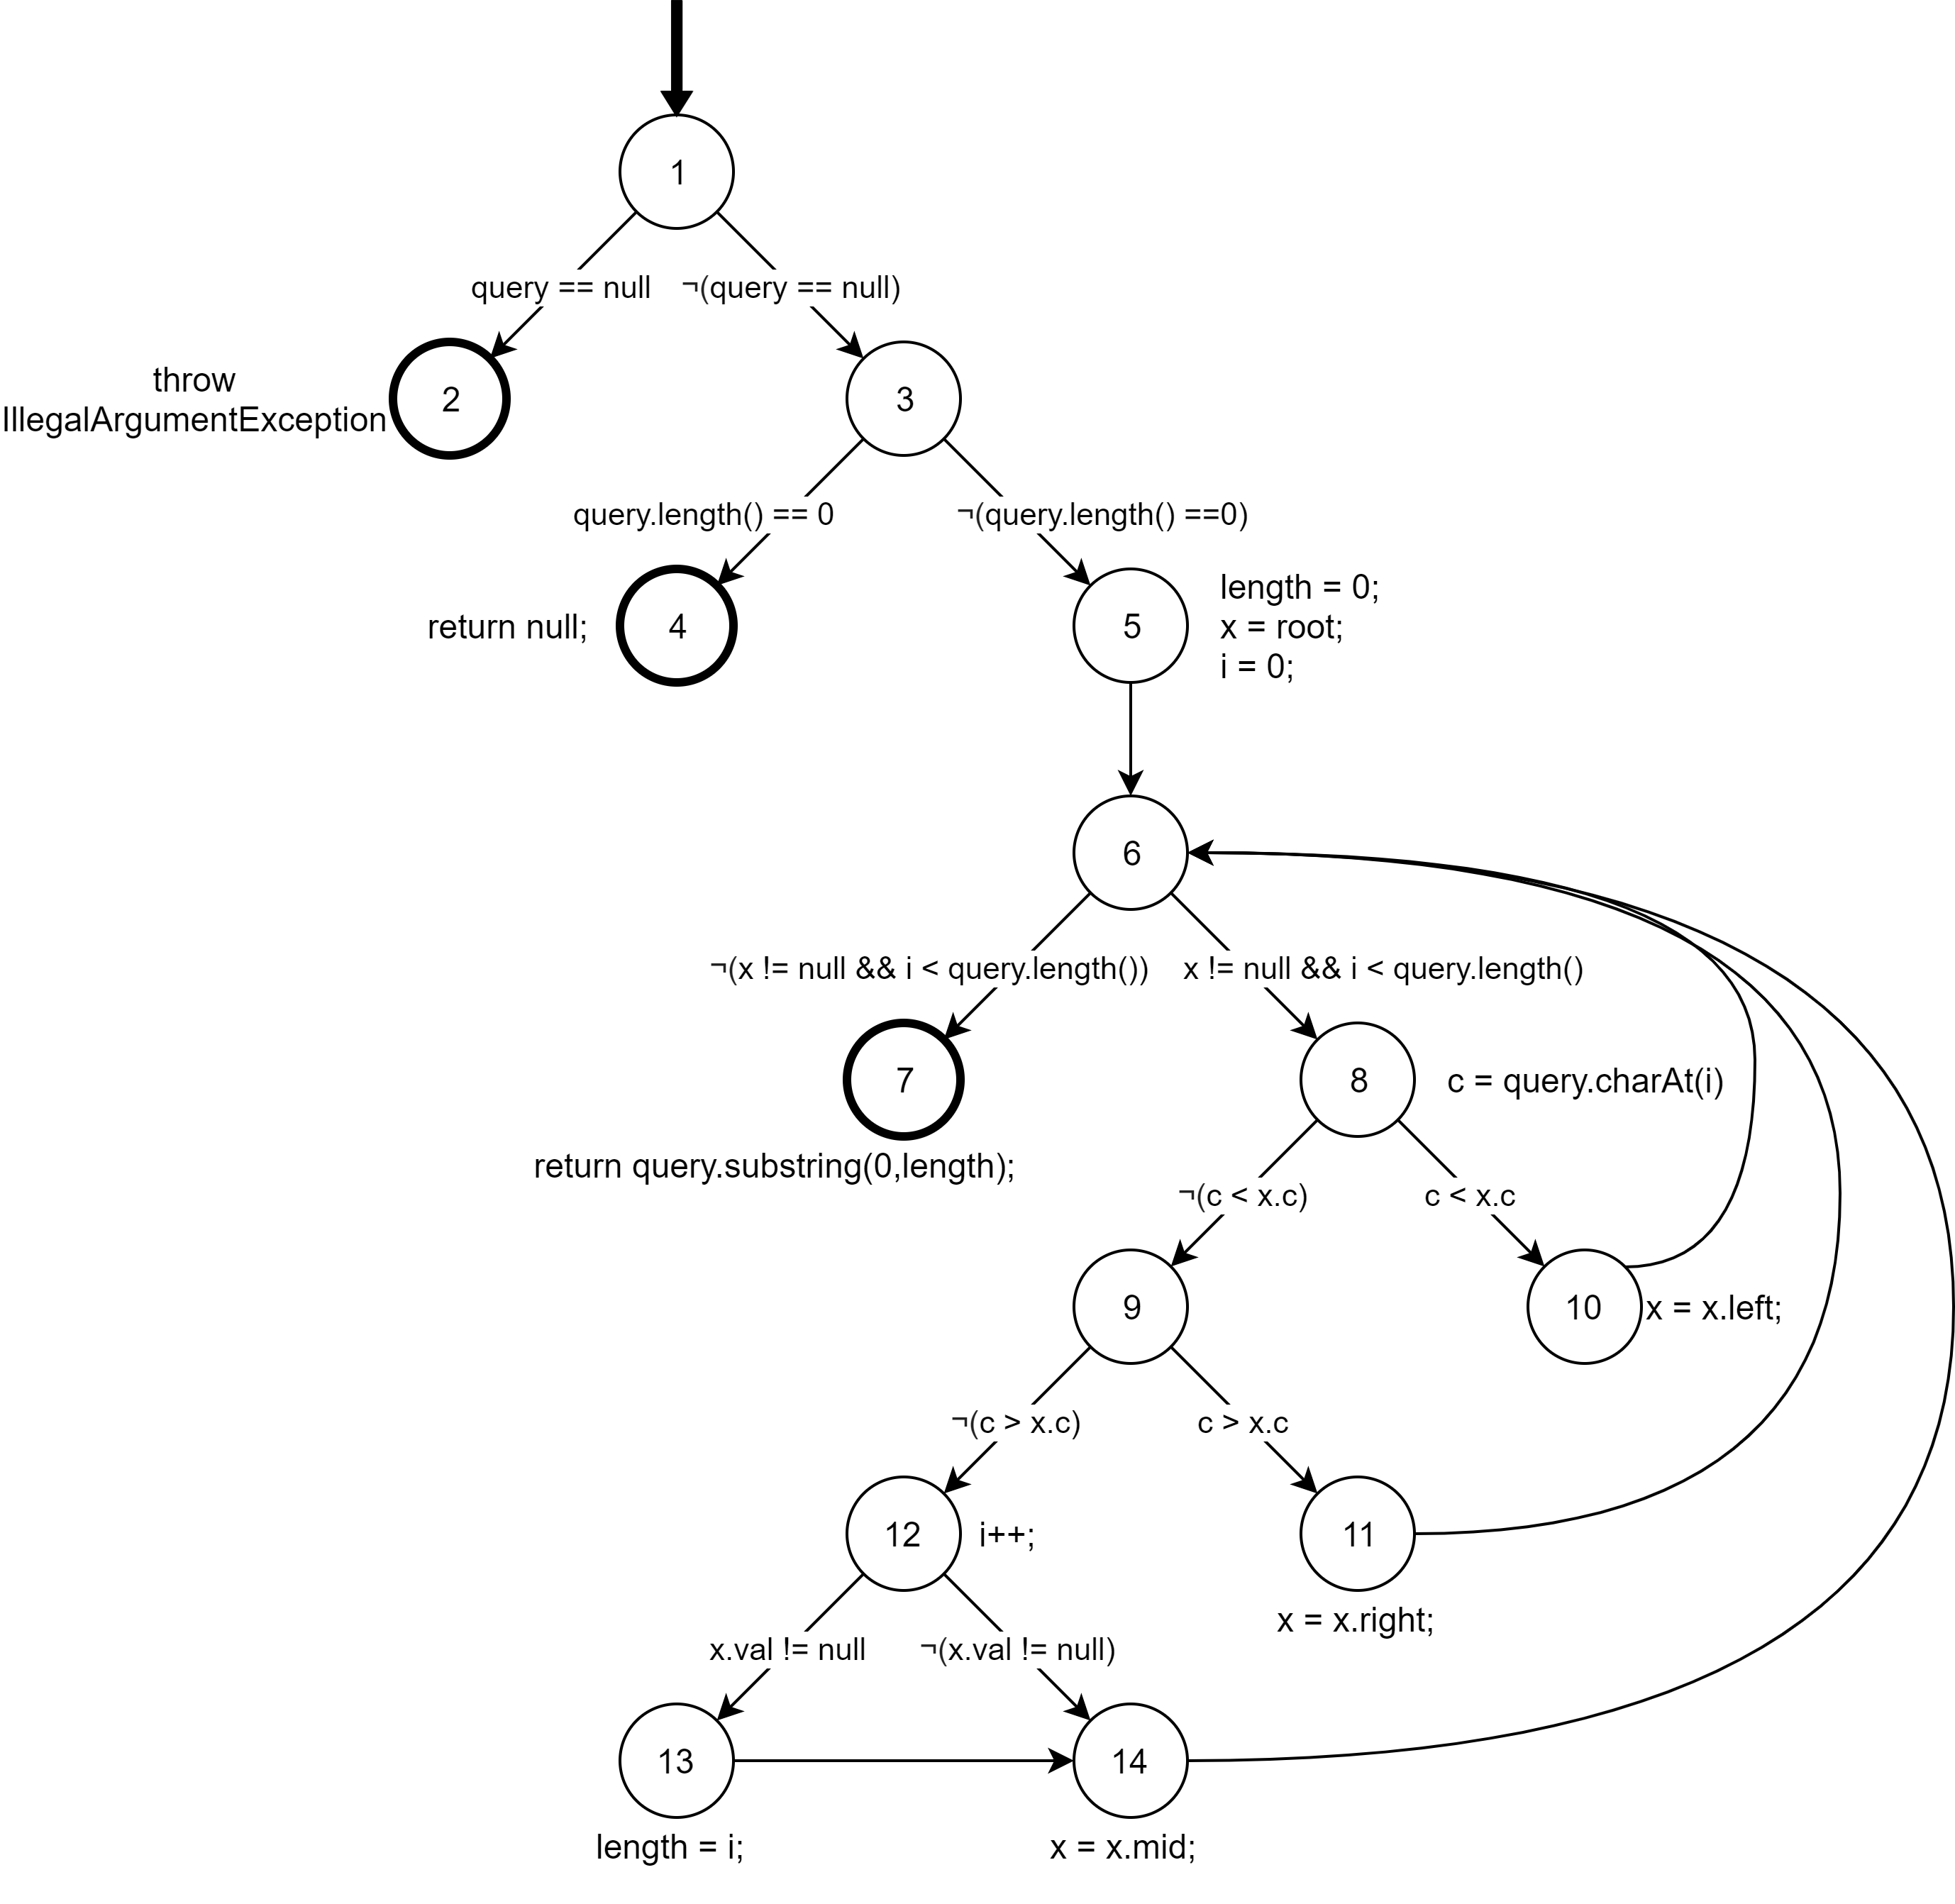
\includegraphics[scale=0.15]{longestPrefixOfGraph.png}
  	\caption{longestPrefixOf's Graph}
\end{figure}


\section{Prime Path Coverage}



\section{All-Uses Coverage }

\begin{table}[htb]
\centering
\begin{tabular}{| c | c | c |} 
 \hline
 \textbf{nodes \& edges : I} & \textbf{def(I}) & \textbf{use(I)} \\ \hline
 1                      & \{root, query\} & \{\} \\ \hline
 (1,2), (1,3)           & \{\} & \{query\} \\ \hline
 3                      & \{\} & \{\} \\ \hline
 (3,4), (3,5)           & \{\} & \{query\} \\ \hline
 4                      & \{\} & \{\} \\ \hline
 5                      & \{length, x, i\} & \{root\} \\ \hline
 (5,6)                  & \{\} & \{\} \\ \hline
 6                      & \{\} & \{\} \\ \hline
 (6,7), (6,8)           & \{\} & \{x, i, query\} \\ \hline
 7                      & \{\} & \{query, length\} \\ \hline
 8                      & \{c\} & \{i\} \\ \hline
 (8,9), (8,10)          & \{\} & \{c, x\} \\ \hline
 9                      & \{\} & \{\} \\ \hline
 10                     & \{x\} & \{x\} \\ \hline
 (10,6), (11,6), (14,6) & \{\} & \{\} \\ \hline
 (9,11), (9,12)         & \{\} & \{c, x\} \\ \hline
 12                     & \{x\} & \{x\} \\ \hline
 12                     & \{i\} & \{i\} \\ \hline
 (12,13), (12,14)       & \{\} & \{x\} \\ \hline
 13                     & \{length\} & \{i\} \\ \hline
 14                     & \{x\} & \{x\} \\ \hline
\end{tabular}
\end{table}

\begin{table}[htb]
\centering
\begin{tabular}{| c | c | c |} 
 \hline
 \textbf{var} & \textbf{node} & \textbf{du(node,var)} \\ \hline
 query        & 1 & [1,2], [1,3], [1,3,4], [1,3,5], [1,3,5,6,7], [1,3,5,6,8] \\ \hline
 root         & 1 & [1,3,5] \\ \hline
 length       & 5 & [5,6,7] \\ \hline
 length       & 13 & [13,14,6,7] \\ \hline
 x            & 5 & \makecell{[5,6,7], [5,6,8], [5,6,8,10], [5,6,8,9], [5,6,8,9,11] \\\ [5,6,8,9,12], [5,6,8,9,12,13], [5,6,8,9,12,13,14], [5,6,8,9,12,14]} \\ \hline
 x            & 10 & \makecell{[10,6,7], [10,6,8], [10,6,8,10], [10,6,8,9] \\\ [10,6,8,9,11], [10,6,8,9,12], [10,6,8,9,12,13] \\\ [10,6,8,9,12,13,14], [10,6,8,9,12,14]} \\ \hline
 x            & 11 & \makecell{[11,6,7], [11,6,8], [11,6,8,10], [11,6,8,9] \\\ [11,6,8,9,11], [11,6,8,9,12], [11,6,8,9,12,13] \\\ [11,6,8,9,12,13,14], [11,6,8,9,12,14]} \\ \hline
 x            & 14 & \makecell{[14,6,7], [14,6,8], [14,6,8,10], [14,6,8,9] \\\ [14,6,8,9,11], [14,6,8,9,12], [14,6,8,9,12,13] \\\ [14,6,8,9,12,13,14], [14,6,8,9,12,14]} \\ \hline
 i            & 5 & [5,6,7], [5,6,8], [5,6,8,9,12], [5,6,8,9,12,13] \\ \hline
 i            & 12 & \makecell{[12,13], [12,13,14,6,7], [12,13,14,6,8] \\\ [12,13,14,6,8,9,12], [12,14,6,7], [12,14,6,8], [12,14,6,8,9,12]} \\ \hline
 c            & 8 & [8,9], [8,10], [8,9,11], [8,9,12] \\ \hline
\end{tabular}
\end{table}


\section{Logic-based Coverage}





\begin{thebibliography}{9}
\bibitem{silk} 
SiLK - CERT NetSA
\url{https://tools.netsa.cert.org/silk/docs.html}

\bibitem{ports} 
List of TCP and UDP port numbers
\url{https://en.wikipedia.org/wiki/List_of_TCP_and_UDP_port_numbers}



\end{thebibliography}


\bibliographystyle{plain}
\end{document}

%%% Local Variables:
%%% mode: latex
%%% TeX-master: t
%%% End:
